\documentclass[conference]{IEEEtran}
\hyphenation{op-tical net-works semi-conduc-tor IEEEtran}
\usepackage[bottom=2cm,top=3cm,left=3cm,right=2cm]{geometry}
\usepackage{url}
\makeatletter
\def\ps@pprintTitle{%
	\let\@oddhead\@empty
	\let\@evenhead\@empty
	\def\@oddfoot{\reset@font\hfil\thepage\hfil}
	\let\@evenfoot\@oddfoot
}
\makeatother

\usepackage{babelbib}

\usepackage[brazilian]{babel} % Traduz alguns termos para o português
\usepackage[utf8]{inputenc} % Reconhece acentuação
\usepackage{setspace}
\usepackage{graphicx}


\begin{document}

% paper title
\title{Teoria da Decisão\\ Métodos Escalares de Otimização Vetorial e Tomada de Decisão Assistida}


% author names and affiliations
% use a multiple column layout for up to three different
% affiliations
\author{\IEEEauthorblockN{Rafael Carneiro de Castro}
\IEEEauthorblockA{\\Engenharia de Sistemas - UFMG\\
Matrícula: 2013030210\\
Email: rafaelcarneiroget@hotmail.com}
\and
\IEEEauthorblockN{Davi Pinheiro Viana}
\IEEEauthorblockA{\\Engenharia de Sistemas - UFMG\\
	Matrícula: 2013029912\\
	Email: daviviana22@gmail.com}}

\maketitle

\begin{abstract}
Abordagem de forma conjunta de grande parte dos conceitos vistos na disciplina "ELE088 - Teoria da Decisão", através de um problema de escalonamento de tarefas. O problema foi resolvido através de implementações mono e multiobjetivo e utilizando o método de auxílio à tomada de decisão Programação de Compromissos.
\end{abstract}

\IEEEpeerreviewmaketitle

\section{Introdução}
O presente trabalho tem o objetivo de resolver um problema de otimização, utilizando técnicas escalares de decisão assistida, estudadas em sala de aula, e colocar em prática grande parte dos conceitos da matéria.

O problema a ser resolvido é o seguinte:
\textit{Uma empresa possui um conjunto de M máquinas que devem ser utilizadas para processar N tarefas indivisíveis. Cada máquina $i$ leva um tempo $t_{ij}$ para processar uma tarefa $j$ e pode processar uma única tarefa por vez. Todas as tarefas possuem uma mesma data ideal de entrega $d$, sendo que cada tarefa $j$ sofre uma penalidade $w_j$ proporcional a cada dia que ela é entregue adiantada ou atrasada em relação a $d$.}

Deve ser feita a formulação e resolução do problema nas versões mono e multiobjetivo e também utilização da técnica de análise de decisão \emph{Programação de Compromissos}.

\section{Desenvolvimento}
\subsection{Formulação do Problema:}
A formulação do problema foi dividida em duas partes, como é discutido a seguir:

\subsubsection{Minimização do Tempo Total de Entrega}
Em primeiro momento, é preciso construir uma função objetivo e suas eventuais restrições para minimização do tempo total de entrega de todas as tarefas. Considere $C_i$ como sendo o tempo necessário para se terminar as tarefas executadas pela máquina $i$. Assim:
\[C_i = \sum_{j=1}^{N}t_{ij} \cdot x_{ij}\ \forall\ i \in\ (1,...,M) \]
O objetivo então se torna:
\[\mathrm{min}\ C_{\mathrm{max}} \]
\[C_{\mathrm{max}} = \mathrm{max}(C_i)\ \forall\ i \in\ (1,...,M) \]
sujeito a:

\begin{equation}
	\sum_{i=1}^{N}x_{ij}=1\ \forall\ j \in\ (1,...,M)
	\label{eq:rest1}
\end{equation}
\[ x_{ij} \in (0, 1)\]

A restrição contida na equação \ref{eq:rest1}, garante que todas as tarefas serão cumpridas e, também, que cada tarefa será executada por uma única máquina. A matriz $x$ é composta por zeros e uns. Cada uma das suas linhas, então, vai representar uma tarefa, e cada coluna, uma máquina. O número 1 em uma coluna representa qual máquina vai executar a tarefa daquela linha.

\subsubsection{Minimização da Soma Ponderada dos Atrasos e Adiantamentos}
Agora, uma função objetivo para tratar a minimização da soma ponderada dos atrasos e adiantamentos é formulada. O momento de término da tarefa $j$ será chamado de $e_j$. Então:
\[e_j = \sum{}{}t_{ik}\ \forall\ k \in\ \Omega_j \]
onde $\Omega_j$ é o conjunto das tarefas até a tarefa $j$ executadas por uma mesma máquina $i$. A função objetivo pode ser escrita como:
\[\mathrm{min}\ \sum_{j=1}^{N}w_j|e_j-d| \]
sujeito a:
\begin{equation}
\sum_{i=1}^{M}x_{ij}=1\ \forall\ j \in\ (1,...,N)\\
\label{eq:rest3}
\end{equation}
\[x_{ij} \in (0, 1)\]

onde, como já discutido, $d$ é a data ideal de entrega das tarefas e $w_j$ a penalidade proporcional a cada dia que a tarefa é entregue adiantada ou atrasada em relação a $d$.

A restrição contida na equação \ref{eq:rest3}, garante que todas as tarefas serão cumpridas e, também, que cada tarefa será executada por uma única máquina

\subsection{Algoritmos de Solução:}
Nesta seção serão discutidos e exibidos os algoritmos para solução dos problemas mono e multiobjetivo.
\subsubsection{Minimização do Tempo Total de Entrega}
O algoritmo de otimização utilizado aqui se baseia no \textit{Simulated Annealing} (SA), método estudado em sala de aula de fácil implementação e convergência atrativa. Este método escapa de mínimos locais com a aceitação de alguns movimentos de piora na qualidade da solução. É inspirado no recozimento físico de sólidos, e possui um parâmetro conhecido como \textit{temperatura}, que ajusta a probabilidade de um movimento de piora ser aceito. Um algoritmo simplificado para o \textit{Simulated Annealing} pode ser visto na Figura \ref{fig:algoritmo}.

	\begin{figure}[h]
%		\centering
		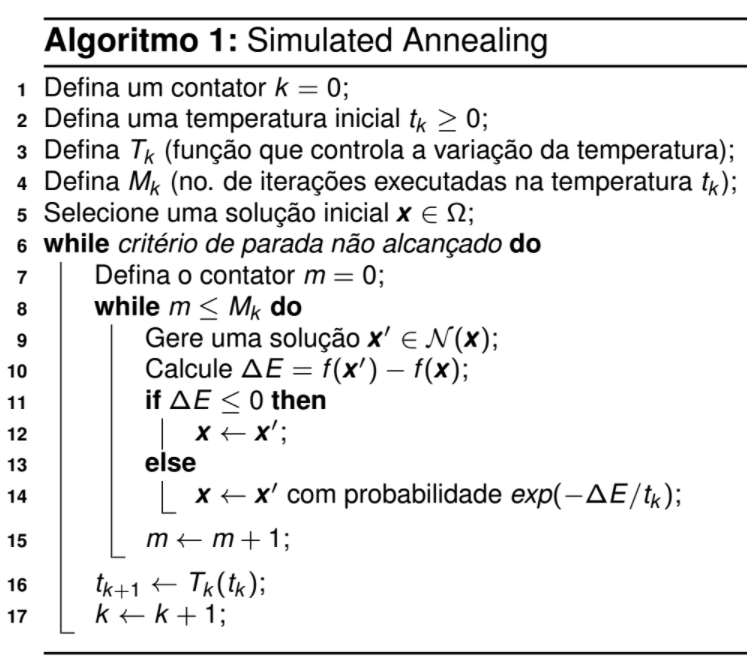
\includegraphics[width=8cm]{img/sa.png}
		\caption{Algoritmo simplificado do SA.}
		\label{fig:algoritmo}
	\end{figure}
	
Para tratar o problema da minimização do tempo de entrega, é importante ter em mente a representação de uma possível solução. Esta representação, como discutido na seção A.1, é uma matriz de zeros e uns, onde o 1 representa qual máquina faz dada tarefa.

A primeira etapa foi criar um algoritmo que gera uma solução inicial. Este código está no arquivo \texttt{initialSolTE.m}. Uma solução é inicializada como sendo uma matriz de zeros. Então, para cada linha (tarefa), um número randômico entre 1 e a quantidade de máquinas é gerado, representado qual é a máquina escolhida para executar a tarefa daquela linha. Um número 1 é colocado na posição da linha do número randômico gerado. Repare que esta solução gerada nunca viola a restrição de que a soma dos valores de uma linha deve ser sempre 1.

Em seguida, criou-se um código que é responsável por avaliar uma dada solução na função objetivo, algoritmo este que está no arquivo \texttt{fobjTE.m}. Este arquivo define a função \emph{fobjTE} que recebe como entrada a solução que se deseja avaliar e uma matriz com o tempo que cada máquina demora para executar cada tarefa (estes tempos são carregados do arquivo \texttt{i5x25.mat} disponibilizado pelo professor). Pela multiplicação vetorial de cada linha da matriz dos tempos com cada coluna da matriz $x$ (solução), tem-se o tempo de operação de cada máquina. A avaliação da solução na função objetivo é, como já visto, o maior dentre os tempos de operação das máquinas.

Antes de implementar o SA propriamente dito, foi necessário também criar funções que geram novas soluções em dada vizinhança. Para este problema, duas funções de vizinhança foram criadas. A primeira, para uma dada solução $x$, gera uma nova solução $y$ trocando aleatoriamente as máquinas que executam $n$ tarefas ($n$ também é um parâmetro da função), e está no arquivo \texttt{neighbor1TE.m}. Repare que aqui não ocorre necessariamente uma troca entre máquinas. A outra função de vizinhança recebe uma solução $x$ e gera uma nova solução $y$ escolhendo duas linhas aleatoriamente (duas tarefas), e trocando-as, de forma que duas máquinas trocam as tarefas entre si. Está no arquivo \texttt{neighbor2TE.m}. Com estas funções de vizinhança, a restrição de que cada linha pode ter apenas um número 1 (cada tarefa só pode ser executada por uma máquina) ainda é atendida.

O algoritmo de otimização foi implementado no arquivo \texttt{minTempoEntrega.m}, que tem a função de mesmo nome. Utiliza a estratégia do \textit{Simulated Annealing} e também, como auxílio, todos os outros algoritmos apresentados até aqui para o problema em questão. A função \textit{minTempoEntrega} implementada no arquivo possui dois argumentos, o que vai facilitar, posteriormente, no ajuste de parâmetros do método implementado. Este ajuste será apresentado na seção de resultados.

\subsubsection{Minimização da Soma Ponderada dos Atrasos e Adiantamentos}
O algoritmo de otimização utilizado aqui também se baseia no \textit{Simulated Annealing}, ilustrado na Figura \ref{fig:algoritmo}.

Para a representação de uma possível solução, a estrutura de dados é dividida em duas partes. Uma delas é a própria matriz $x$ usada no primeiro problema e discutida na seção A.1. Esta matriz contém as informações de qual máquina executa as tarefas. A informação adicional que este problema exige é a ordenação das tarefas em cada máquina. Por questão de simplicidade de código, as tarefas receberam a ordem em um único vetor, com todas as 25. Se uma tarefa antecede a outra neste vetor, mas elas não são da mesma máquina, não significa que uma começou a ser executada antes que a outra, já que elas são de máquinas diferentes. A ordem só vai ser importante quando se olhar as tarefas de uma mesma máquina. 

Para a geração de uma solução inicial, cria-se uma matriz $x$ com a chamada do código que está em \texttt{initialSolTE.m}, que é o código do exemplo anterior. Agora, para se gerar uma ordenação, basta chamar a função $randperm$ do MatLAB, para criar uma permutação randômica de 1 até N, onde N é a quantidade de tarefas. Tanto $x$ quanto a ordem são retornados pela função, que está no arquivo \texttt{initialSolSPA.m}.

Em seguida, criou-se um código que é responsável por avaliar uma dada solução na função objetivo, algoritmo este que está no arquivo \texttt{fobjSPA.m}. Este arquivo define a função \emph{fobjSPA} que recebe como entrada: a solução (matriz $x$) que se deseja avaliar, um vetor contendo a ordem de execução das tarefas, uma matriz com o tempo que cada máquina demora para executar cada tarefa, um vetor com o custo do atraso ou adiantamento de cada tarefa, e o dia de entrega ótimo das tarefas. Estes dados são carregados do arquivo \texttt{i5x25.mat} disponibilizado pelo professor. Todas as tarefas de uma dada máquina são percorridas e o tempo de término de cada uma é calculado, adicionando ao resultado final a penalidade proveniente de cada tarefa.

Antes de implementar o SA propriamente dito, foi necessário também criar funções que geram novas soluções em dada vizinhança. Para este problema, três funções de vizinhança foram criadas.

A primeira, para uma dada solução $x$, gera uma nova solução $y$ trocando, aleatoriamente, a máquina que executa uma determinada tarefa. A implementação dessa estrutura de vizinhança está no arquivo \texttt{neighbor1SPA.m}. Repare que aqui não ocorre necessariamente uma troca entre as máquinas sendo que, na nova solução gerada, uma das máquinas pode ficar sem executar nenhuma tarefa, por exemplo.

A outra função de vizinhança recebe uma solução $x$ e gera uma nova solução $y$, trocando a ordem de duas tarefas aleatórias, em uma mesma máquina, escolhida também de maneira aleatória. A implementação dessa estrutura está no arquivo \texttt{neighbor2SPA.m}.

A última função de vizinhança troca todas as tarefas de duas máquinas entre si, não alterando a ordem que elas são executadas na máquina. Nessa estrutura, se certo número de estágios estagnados for alcançado, são geradas soluções mais espaçadas de forma a explorar uma região mais distante. A implementação encontra-se no arquivo \texttt{neighbor3SPA.m}

Em todas as estruturas de vizinhança criadas, a restrição de que cada linha pode ter apenas um número 1 (cada tarefa só pode ser executada por uma máquina) é atendida.

O algoritmo de otimização foi implementado no arquivo \texttt{minAtrasoAdiantamento.m}, que tem a função de mesmo nome. Utiliza a estratégia do \textit{Simulated Annealing} e também, como auxílio, todos os outros algoritmos apresentados até aqui para o problema em questão. A função \textit{minAtrasoAdiantamento} implementada no arquivo possui um argumento, o que vai facilitar, posteriormente, no ajuste de parâmetros do método implementado. Este ajuste será apresentado na seção de resultados.

\subsubsection{Otimização multiobjetivo - Soma ponderada}
Uma versão de resolução do problema apontado anteriormente é a otimização dos dois objetivos ao mesmo tempo (multiobjetivo). Ou seja, ao mesmo tempo em que se minimiza o \emph{tempo total de entrega}, minimiza-se também a \emph{soma ponderada dos atrasos e adiantamentos}. Essa versão do problema é mais próxima da situação real em que sempre se busca os dois objetivos.

O primeiro método  aplicado para resolução da versão mutiobjetivo foi a \emph{Soma Ponderada}. Nele, as duas funções objetivos são agrupadas em uma única função. A nova função objetivo é composta de um somatório ponderado das funções anteriores e as restrições são as mesmas dos dois problemas. Assim, a função objetivo transformada se torna a seguinte:

\[\mathrm{min}\ p_1 \cdot C_{\mathrm{max}} + p_2 \cdot \left( \sum_{j=1}^{N}w_j|e_j-d| \right)\]
sujeito a:
\begin{equation}
\sum_{i=1}^{M}x_{ij}=1\ \forall\ j \in\ (1,...,N)
\label{eq:rest4}
\end{equation}
\[x_{ij} \in (0, 1)\]
\[p_1 \ge 0\]
\[p_2 \ge 0\]
\[p_1 + p_2 = 1\]

Em que $p_1$ e $p_2$ são os pesos dados às funções objetivos originais. A função objetivo transformada pode ser resolvida por qualquer método de otimização não linear.

No trabalho, foi utilizado um algoritmo também baseado no \emph{Simulated Annealing}, já citado anteriormente. Tanto para geração de solução inicial, como para estruturas de vizinhança, foram utilizados os mesmos métodos implementados para resolução da \emph{Soma ponderada dos atrasos e adiantamentos}. Os métodos foram reutilizados por se tratarem da mesma estrutura de algoritmo e por gerarem solução e vizinhança que atendem aos dois problemas.

No algoritmo, primeiramente é gerada uma solução inicial utilizando a função presente no arquivo \texttt{initialSolSPA.m}. Após, é repetido o seguinte processo: gera-se valores aleatórios de $p_1$ e $p_2$ e resolve-se o problema da  função transformada utilizando algoritmo SA. A solução pareto-ótima encontrada é armazenada. Foi feita implementação para que sejam encontradas 100 (cem) soluções por execução do algoritmo.

O método da soma ponderada foi escolhido por ser simples e fácil de programar e, também, pelo fato da função transformada possuir apenas dois objetivos, já que, para o método da solução ponderada, não são indicadas funções com muitos objetivos pela dificuldade de controlar a diversidade das soluções encontradas. A implementação da resolução do problema pode ser encontrada no arquivo \texttt{somaPonderada.m}. Nele, foi criada a função \emph{somaPonderada} que recebe os mesmos parâmetros da função \emph{minTempoEntrega} para o ajuste de parâmetros.

\subsubsection{Otimização multiobjetivo - $\epsilon$-restrito}

O segundo método aplicado para resolução da versão multiobjetivo foi o \emph{$\epsilon$-restrito}. Nele, escolhe-se uma das funções objetivos para se minimizar e as demais se tornam restrições de desigualdade para o problema transformado. No trabalho, foi escolhido minimizar a função \emph{somatório dos atrasos e adiantamentos} e a função \emph{tempo total de entrega} se tornou uma restrição. Assim, a função objetivo transformada se tornou a seguinte:

\[\mathrm{min}\ \sum_{j=1}^{N}w_j|e_j-d| \]
sujeito a:
\begin{equation}
C_{\mathrm{max}} \le \epsilon_1
\end{equation}
\begin{equation}
\sum_{i=1}^{M}x_{ij}=1\ \forall\ j \in\ (1,...,N)\\
\label{eq:rest6}
\end{equation}
\[x_{ij} \in (0, 1)\]

A função objetivo transformada pode ser resolvida por qualquer método de otimização não linear. No trabalho, foi utilizado novamente um algoritmo baseado no \emph{Simulated Annealing} (SA), já citado anteriormente. Assim como na \emph{Soma ponderada}, foram utilizados os métodos de geração de solução inicial e de vizinhança do método da \emph{Soma dos atrasos e adiantamentos}.

O algoritmo gera uma solução inicial e repete o método SA para encontrar o conjunto de soluções pareto-ótimas, variando o valor de $\epsilon_1$. No trabalho foram encontradas 100 (cem) soluções por execução do algoritmo.

Esse método foi escolhido por ser mais robusto que a \emph{Soma Ponderada} e pelo fato de se ter apenas dois objetivos, já que o \emph{$\epsilon$-restrito}, para resolução de problemas com mais de dois objetivos, pode gerar funções transformadas infactíveis. A implementação da resolução do problema pode ser encontrada no arquivo \texttt{epsilonRestrito.m}.

\subsubsection{Programação de Compromisso}
Além dos métodos utilizados para resolver o problema multiobjetivo, foi implementado o método \emph{Programação de Compromisso}. Essa é uma técnica de análise de decisão multicritério que visa encontrar a melhor solução de compromisso para um problema de otimização com múltiplos objetivos.

A análise para encontrar a solução de compromisso consiste no decisor definir valores aceitáveis para as funções objetivo do problema e então, é feita a minimização encontrando soluções que atendam aos valores definidos.

Para aplicar a técnica, foi feita a seguinte transformação no problema multiobjetivo:

\[ \mathrm{min} {\left[ w_1 \cdot {| f_1(x) - f_1^{*} |}^{r} + w_2 \cdot {| f_2(x) - f_2^{*} |}^{r} \right]}^{\frac{1}{r}} \]

sujeito a
\begin{equation}
\sum_{i=1}^{M}x_{ij}=1\ \forall\ j \in\ (1,...,N)
\label{eq:rest5}
\end{equation}

\[1 \le r \le \infty \]

Em que $w_1$ e $w_2$ são pesos que caracterizam a preferência do decisor, $f_1(x)$ é a função objetivo do problema do \emph{Tempo Total de entrega}, $f_2(x)$ é a função objetivo do problema da \emph{Soma Ponderada dos Atrasos e Adiantamentos}, $r$ é um parâmetro variável que define se será feita a minimização da soma dos desvios ou do máximo desvio e $f_{1}^*$ e $f_{2}^{*}$ são parâmetros que o decisor define como sendo valores aceitáveis das funções objetivos. No caso do problema a ser resolvido, $f_1^*$ define o tempo total de entrega aceitável e $f_2^*$ define a soma ponderada dos atrasos e adiantamentos aceitável.

A função da \emph{Programação de Compromisso} também pode ser resolvida por qualquer método de otimização não linear e para resolução dela foi utilizado o algoritmo baseado no \emph{Simulated Annealing}. Também foram utilizados os métodos de geração de solução inicial e de vizinhança do método da \emph{Soma dos atrasos e adiantamentos}.

O algoritmo gera uma solução inicial e repete o método SA para encontrar o conjunto de soluções pareto-ótimas variando os valores de $w_1$ e $w_2$. Foi feita essa implementação pelo fato dos alunos não terem conhecimento suficiente do problema para escolher valores de pesos precisos para o problema. Além disso, baseado nas execuções dos métodos \emph{Soma Ponderada} e \emph{$\epsilon$-restrito} foi escolhido o valor de $14$ para o parâmetro $f_1^*$ e $400$ para o parâmetro $f_2^*$. Esses parâmetros podem ser facilmente alterados no arquivo com a implementação do algoritmo. O último parâmetro do método é o $r$ que, após algumas execuções do algoritmo, foi escolhido o valor $0,5$. A implementação da \emph{Programação de Compromisso} pode ser encontrada no arquivo \texttt{programacaoDeCompromisso.m}.

\subsection{Resultados:}
Nesta sessão serão apresentados os resultados dos algoritmos.
\subsubsection{Minimização do Tempo Total de Entrega}
Como já mencionado, o algoritmo de otimização foi baseado no \textit{Simulated Annealing}. Esta abordagem exige o ajuste de alguns parâmetros, dentre eles, o multiplicador $\alpha$ de temperatura, que é um valor entre $0$ e $1$, que vai diminuir gradualmente a temperatura do algoritmo: probabilidade de se aceitar um movimento de piora na busca pela melhor solução. Outro parâmetro que deve ser ajustado é a quantidade $n$ de tarefas que terão a máquina aleatoriamente trocada, na primeira função de vizinhança. Os dados para execução do problema foram disponibilizados pelo professor, são carregados pelo arquivo \texttt{i5x25.mat} e podem ser vistos na tabela da Figura \ref{fig:tabela-dados}.

	\begin{figure}[h]
		\centering
		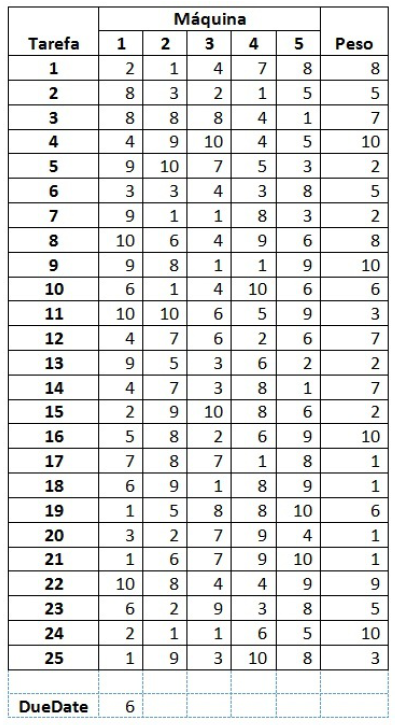
\includegraphics[width=5cm]{img/tabela-dados.png}
		\caption{Tabela de dados para execução dos algoritmos.}
		\label{fig:tabela-dados}
	\end{figure}

Para demonstrar os efeitos da temperatura (parâmetro $\alpha$), uma primeira instancia foi executada, utilizando como parâmetros $\alpha = 0.5$ e $n = 3$. A Figura \ref{fig:result-1} mostra um primeiro resultado desta execução, plotando a avaliação da solução aceita por cada iteração. Como se pode notar, no início do algoritmo, muitas soluções de piora são aceitas, e aos poucos são aceitos, cada vez mais, apenas movimentos de melhora. Esta execução passou por 2141 iterações e a melhor solução encontrada possui avaliação na função objetivo igual a 20.

	\begin{figure}[h]
		\centering
		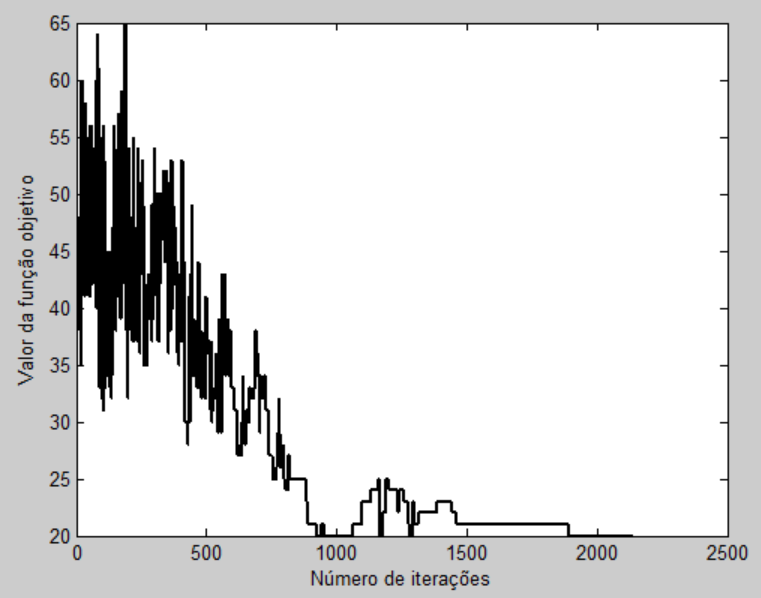
\includegraphics[width=8cm]{img/result-1.png}
		\caption{Primeiro resultado para execução com $\alpha = 0.5$ e $n = 3$.}
		\label{fig:result-1}
	\end{figure}

Executando mais uma vez, mas agora para $\alpha = 0.1$ e $n = 3$, obtemos o resultado mostrado na Figura \ref{fig:result-2}. Como se pode notar, agora menos movimentos de piora são aceitos nas iterações iniciais. Neste caso foram executadas 2488 iterações, com um valor ótimo igual a 14. Ao custo de mais iterações, obteve-se uma ponto de ótimo local melhor.

	\begin{figure}[h]
		\centering
		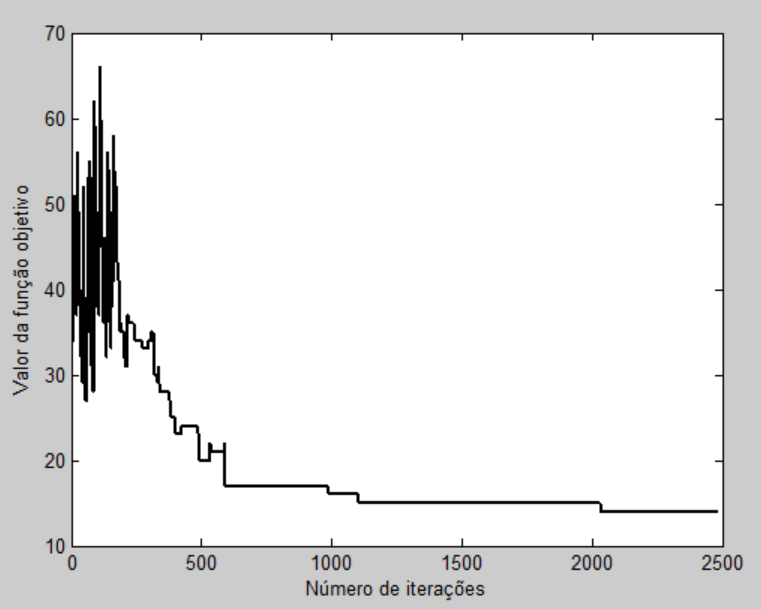
\includegraphics[width=8cm]{img/result-2.png}
		\caption{Primeiro resultado para execução com $\alpha = 0.1$ e $n = 3$.}
		\label{fig:result-2}
	\end{figure}

É necessário então escolher quais serão os parâmetros utilizados, e ainda qual será a função de vizinhança usada. Para tanto, um script de execução foi criado e está no arquivo \texttt{multirunTE.m}. Neste, o código é executado uma quantidade de vezes desejada, e os valores de ótimo e quantidade de iterações para cada execução são plotados. Ajustando o algoritmo para $\alpha = 0.5$ e $n = 3$, após 100 execuções obtemos o resultado mostrado na Figura \ref{fig:mult-result-1}. A linha preta no meio dos gráficos representa a média dos valores. Encontrou-se valor ótimo médio igual a $17,83$ e valor médio da quantidade de iterações igual a $2209,1$.

	\begin{figure}[h]
		\centering
		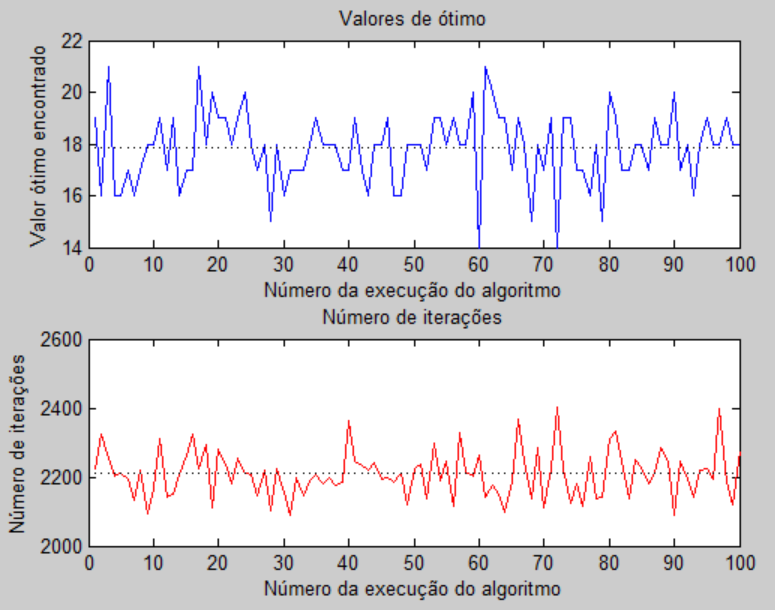
\includegraphics[width=8cm]{img/mult-result-1.png}
		\caption{100 execuções com $\alpha = 0.5$ e $n = 3$.}
		\label{fig:mult-result-1}
	\end{figure}

Foi experimentado também a execução do algoritmo com $\alpha = 0.1$ e $\alpha = 0.01$, ambos mantendo $n = 3$. Os resultados podem ser vistos nas Figuras \ref{fig:mult-result-2} e \ref{fig:mult-result-3}, respectivamente. Para o primeiro caso, a média do valor ótimo foi $14,87$ (com mínimo em $12$ e máximo em $21$) e a média da quantidade de iterações foi $2253,6$ (com mínimo em $2001$ e máximo em $2623$). Para o segundo caso, a média do valor ótimo foi $15,95$ (com mínimo em $13$ e máximo em $19$) e a média da quantidade de iterações foi $2509,4$ (com mínimo em $2299$ e máximo em $2581$). Optou-se então por manter o algoritmo ajustado a $\alpha = 0.1$, por ter uma média de valor ótimo alcançado melhor.

	\begin{figure}[h]
		\centering
		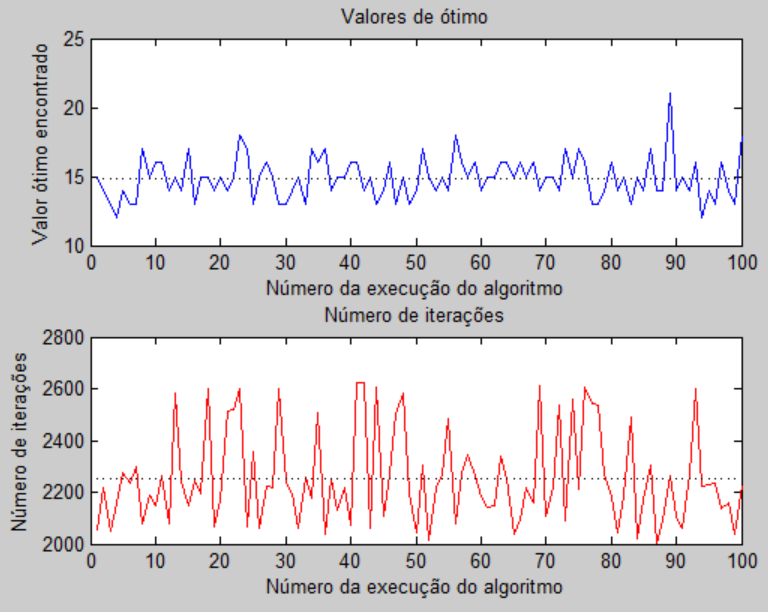
\includegraphics[width=7cm]{img/mult-result-2.png}
		\caption{100 execuções com $\alpha = 0.1$ e $n = 3$.}
		\label{fig:mult-result-2}
	\end{figure}
	
	\begin{figure}[h]
		\centering
		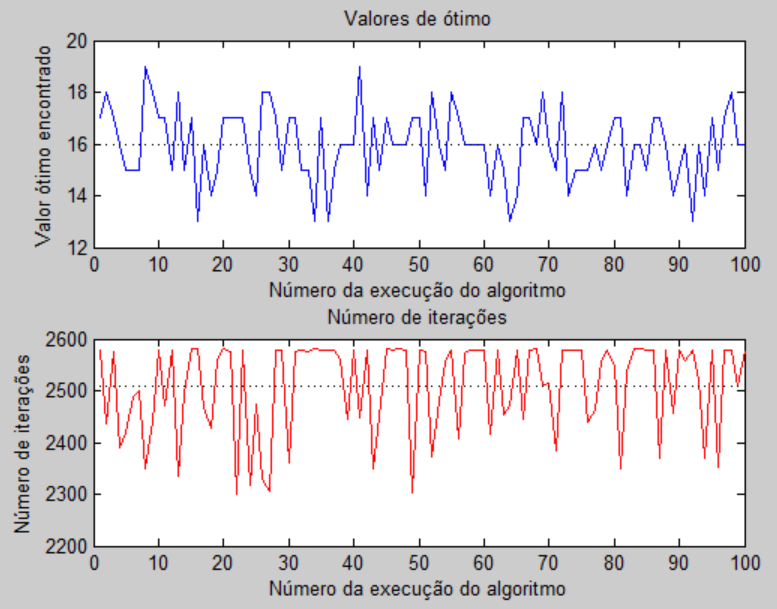
\includegraphics[width=8cm]{img/mult-result-3.png}
		\caption{100 execuções com $\alpha = 0.01$ e $n = 3$.}
		\label{fig:mult-result-3}
	\end{figure}
	\newpage
Como todos estes resultados foram obtidos executando o algoritmo com a primeira forma de vizinhança (\textit{neighbor1TE}), precisamos também decidir um valor para $n$. Mantendo $\alpha = 0.1$, \texttt{multirunTE.m} foi executado para $n = 5$ e $n = 1$. Os resultados podem ser vistos nas Figuras \ref{fig:mult-result-4} e \ref{fig:mult-result-5}, respectivamente. Para o primeiro caso, a média do valor ótimo foi $18,29$ (com mínimo em $15$ e máximo em $22$) e a média da quantidade de iterações foi $2059$ (com mínimo em $2044$ e máximo em $2085$). Para o segundo caso, a média do valor ótimo foi $14,77$ (com mínimo em $12$ e máximo em $20$) e a média da quantidade de iterações foi $2260,8$ (com mínimo em $2003$ e máximo em $2622$). Escolhemos então manter $n = 1$.

	\begin{figure}[h]
		\centering
		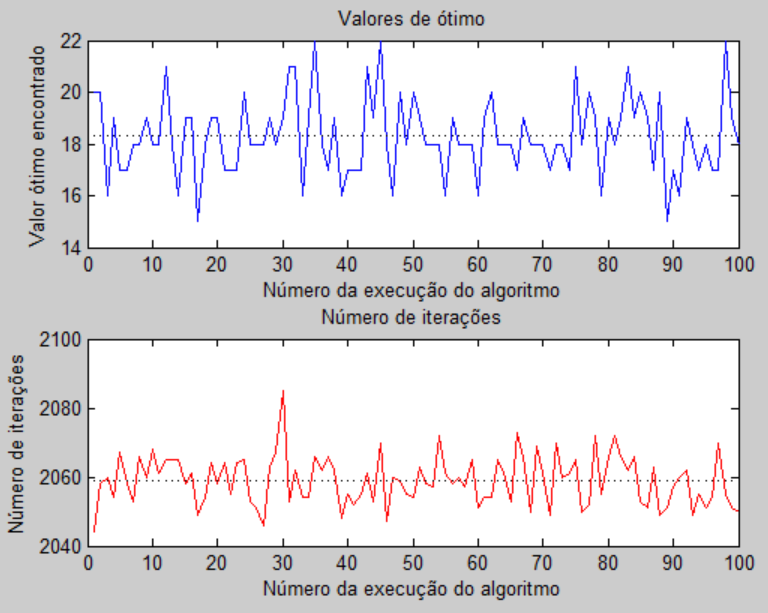
\includegraphics[width=8cm]{img/mult-result-4.png}
		\caption{100 execuções com $\alpha = 0.1$ e $n = 5$.}
		\label{fig:mult-result-4}
	\end{figure}
	
	\begin{figure}[h]
		\centering
		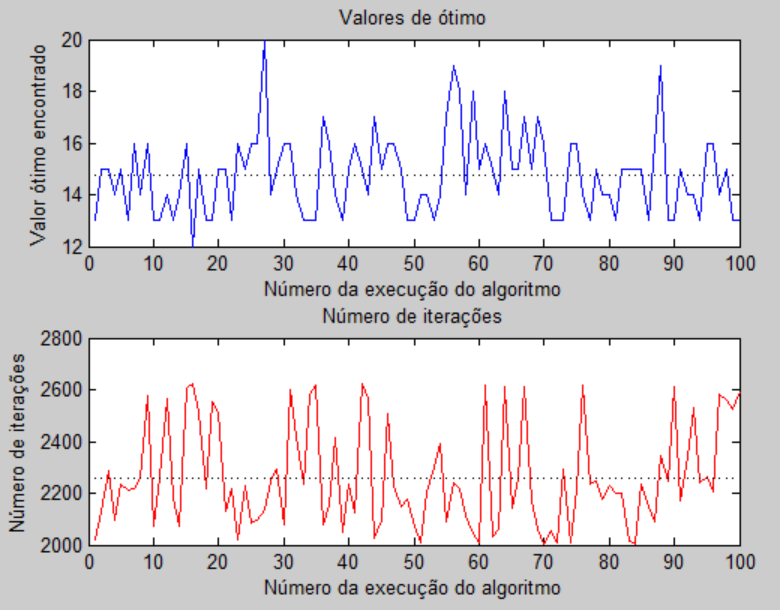
\includegraphics[width=8cm]{img/mult-result-5.png}
		\caption{100 execuções com $\alpha = 0.1$ e $n = 1$.}
		\label{fig:mult-result-5}
	\end{figure}
	\newpage
Todos os resultados vistos até aqui foram com o algoritmo rodando apenas com a função de vizinhança \textit{neighbor1TE}. Agora será incorporado ao algoritmo a função \textit{neighbor2TE} de forma que os dois processos de vizinhança serão executados, um seguido do outro, para se alcançar maior região de busca. Com o auxilio do \texttt{multirunTE.m}, o código foi mais uma vez executado 100 vezes com $\alpha = 0.1$ e $n = 1$, e os resultados podem ser vistos na Figura \ref{fig:mult-result-6}. A média do valor ótimo foi $14,12$ (com mínimo em $12$ e máximo em $16$) e a média da quantidade de iterações foi $2356,5$ (com mínimo em $2043$ e máximo em $2568$). O desempenho foi perceptivelmente melhorado, já que uma maior região de busca é considerada, e melhores ótimos locais são alcançados.

	\begin{figure}[h]
		\centering
		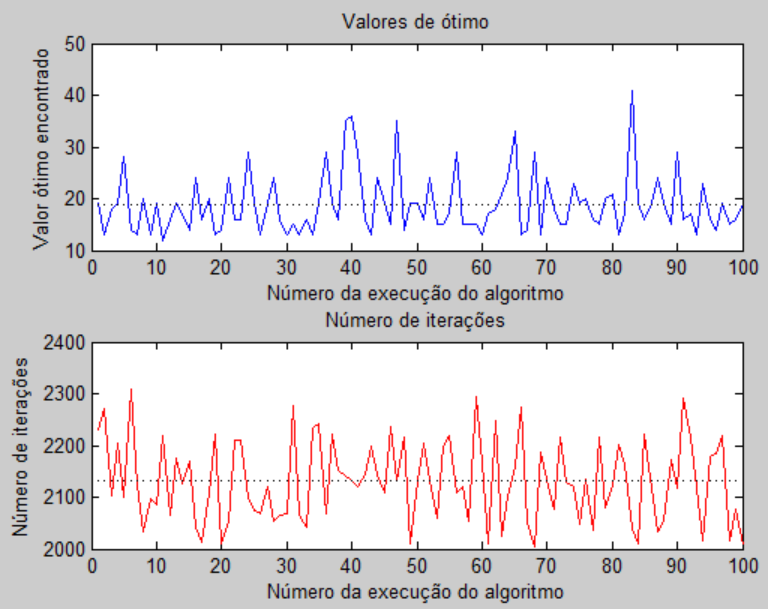
\includegraphics[width=8cm]{img/mult-result-6.png}
		\caption{100 execuções com $\alpha = 0.1$, $n = 1$ e vizinhança \textit{neighbor2TE} adicionada ao código.}
		\label{fig:mult-result-6}
	\end{figure}
	
Com todos os ajustes feitos, o algoritmo foi executado mais 5 vezes, e o resultado sumarizado pode ser visto na Figura \ref{fig:mult-result-7}. Os resultados numéricos são apresentados na Tabela 1.

	\begin{figure}[h]
		\centering
		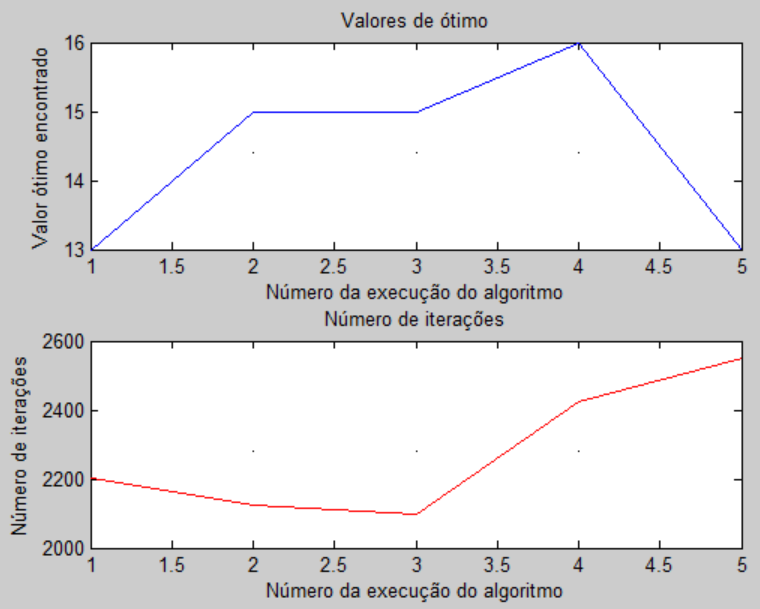
\includegraphics[width=8cm]{img/mult-result-7.png}
		\caption{Resultado final para 5 iterações - Minimização do Tempo de Entrega.}
		\label{fig:mult-result-7}
	\end{figure}
	
	\begin{table}[h]
		\centering
		\begin{tabular}{ | l | l | l | l |}
			\hline
			Ótimo Encontrado & Iterações \\ \hline
			15 & 2336 \\ \hline
			14 & 2440 \\ \hline
			13 & 2392 \\ \hline
			15 & 2228 \\ \hline
			12 & 2330 \\ \hline
		\end{tabular}
		\label{table:result}
		\caption{Resultados numéricos - Minimização do Tempo de Entrega.}
	\end{table}
	
\subsubsection{Minimização da Soma Ponderada dos Atrasos e Adiantamentos}
Para este problema também é necessário fazer o ajuste do parâmetro de temperatura $\alpha$, que é o parâmetro de multiplicação do decaimento da temperatura, como já mencionado. Para ilustrar o efeito deste parâmetro no problema, executou-se uma vez com $\alpha = 0.9$. Vendo na Figura \ref{fig:result-spa-1}, é possível notar que as iterações iniciais do algoritmo permitem muitos movimentos de piora. Agora, se o algoritmo for executado com $\alpha = 0.1$, como pode ser visto na Figura \ref{fig:result-spa-2}, uma menor quantidade de movimentos de piora é aceito, já que a temperatura decai mais rapidamente.

	\begin{figure}[h]
		\centering
		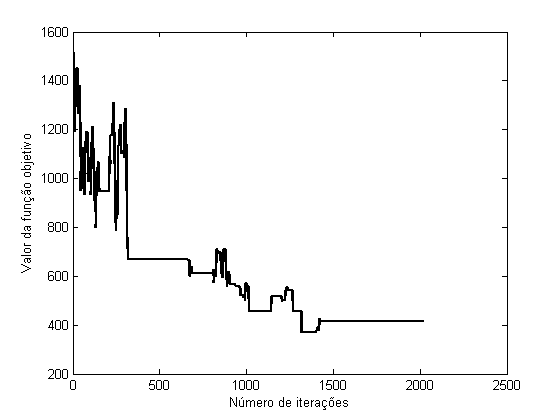
\includegraphics[width=8cm]{img/result-spa-1.png}
		\caption{Primeiro resultado para execução com $\alpha = 0.9$.}
		\label{fig:result-spa-1}
	\end{figure}
	
	\begin{figure}[h]
		\centering
		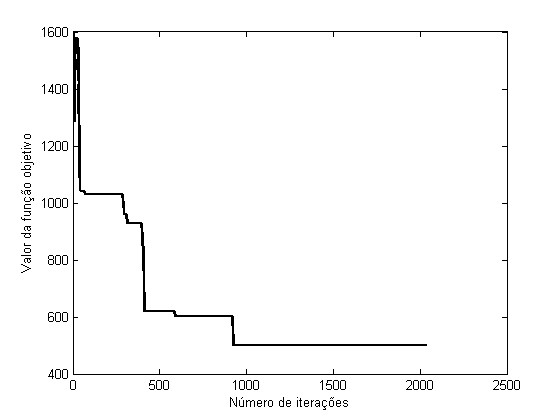
\includegraphics[width=8cm]{img/result-spa-2.png}
		\caption{Primeiro resultado para execução com $\alpha = 0.1$.}
		\label{fig:result-spa-2}
	\end{figure}
	\newpage
Agora para escolher um ajuste de $\alpha$, o algoritmo de otimização do problema foi executado 100 vezes, com auxilio do script \texttt{multirunSPA.m} com $\alpha = 0.1$. O resultado das 100 execuções pode ser visto na Figura \ref{fig:mult-result-spa-1}. A média do valor ótimo foi $580,2$ (com mínimo em $321$ e máximo em $1095$) e a média da quantidade de iterações foi $1893$ (com mínimo em $1397$ e máximo em $2113$).

	\begin{figure}[h]
		\centering
		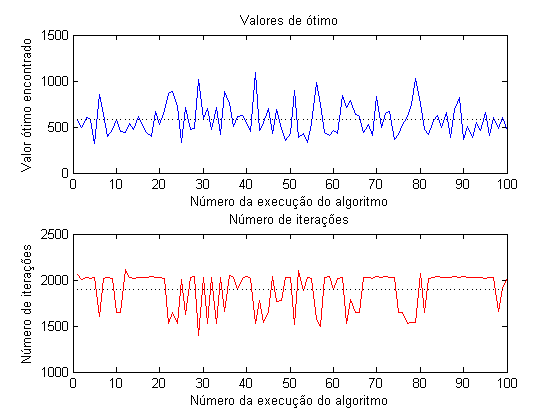
\includegraphics[width=8cm]{img/mult-result-spa-1.png}
		\caption{100 execuções com $\alpha = 0.1$.}
		\label{fig:mult-result-spa-1}
	\end{figure}
	\newpage
Mais uma vez 100 execuções foram feitas, mas com $\alpha = 0.0001$. A Figura \ref{fig:mult-result-spa-2} ilustra os resultados. A média do valor ótimo foi $581,45$ (com mínimo em $357$ e máximo em $1068$) e a média da quantidade de iterações foi $1941,2$ (com mínimo em $1517$ e máximo em $2116$).

	\begin{figure}[h]
		\centering
		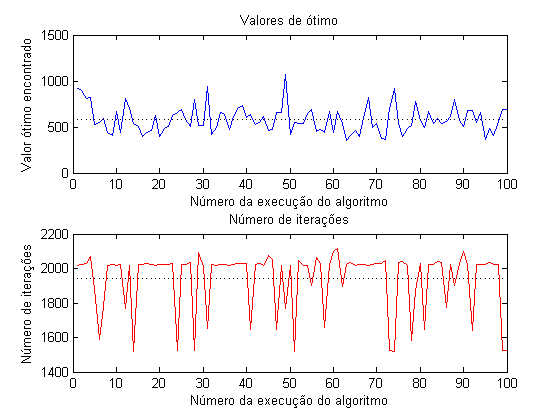
\includegraphics[width=8cm]{img/mult-result-spa-2.png}
		\caption{100 execuções com $\alpha = 0.0001$.}
		\label{fig:mult-result-spa-2}
	\end{figure}
	
Por último, 100 execuções foram feitas com $\alpha = 0.9$. A Figura \ref{fig:mult-result-spa-3} ilustra os resultados. A média do valor ótimo foi $495,6$ (com mínimo em $308$ e máximo em $786$) e a média da quantidade de iterações foi $1895,8$ (com mínimo em $910$ e máximo em $2124$). Com este ajuste de parâmetro, melhor média de valor ótimo foi alcançada, e ainda o teto do ótimo foi reduzido. Por isso, esta será adotada como parametrização final.
	
	\begin{figure}[h]
		\centering
		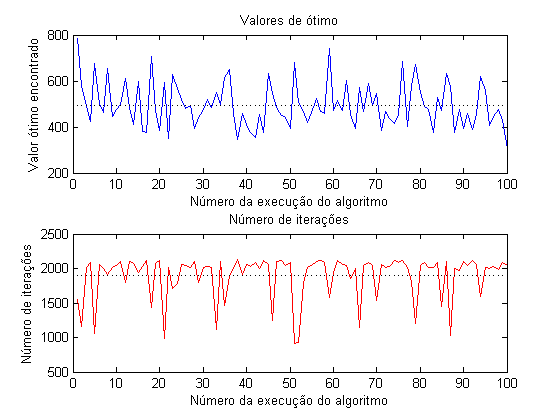
\includegraphics[width=8cm]{img/mult-result-spa-3.png}
		\caption{100 execuções com $\alpha = 0.9$.}
		\label{fig:mult-result-spa-3}
	\end{figure}
	\newpage
Com as decisões de parâmetros tomada, o algoritmo foi executado mais 5 vezes, e o resultado sumarizado pode ser visto na Figura \ref{fig:mult-result-spa-4}. Os resultados numéricos são apresentados na Tabela 2.

	\begin{figure}[h]
		\centering
		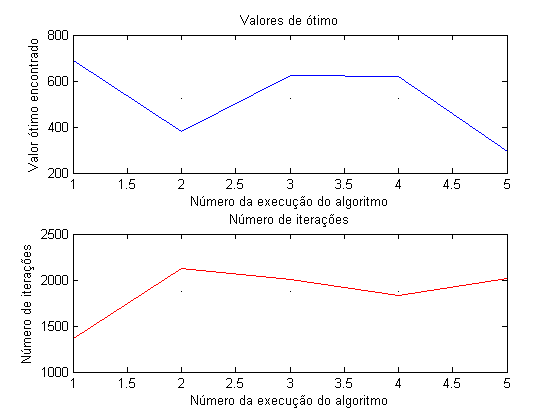
\includegraphics[width=8cm]{img/mult-result-spa-4.png}
		\caption{5 execuções finais com $\alpha = 0.9$.}
		\label{fig:mult-result-spa-4}
	\end{figure}
	
	\begin{table}[h]
		\centering
		\begin{tabular}{ | l | l | l | l |}
			\hline
			Ótimo Encontrado & Iterações \\ \hline
			691 & 1359 \\ \hline
			381 & 2124 \\ \hline
			624 & 2010 \\ \hline
			619 & 1835 \\ \hline
			294 & 2020 \\ \hline
		\end{tabular}
		\label{table:result2}
		\caption{Resultados numéricos - Minimização da Soma Ponderada dos Atrasos e Adiantamentos.}
	\end{table}
	
\subsubsection{Otimização multiobjetivo - Soma ponderada}
Para a execução do algoritmo da Soma Ponderada, presente no arquivo \texttt{somaPonderada.m}, é preciso definir também o valor do parâmetro $\alpha$. Com o histórico das execuções feitas até aqui, e por este ser um algoritmo baseado nos outros, de mesma estrutura e representações, foi decidido usar $\alpha = 0,1$. Conforme dito anteriormente, o script faz a execução do método SA, 100 vezes, variando-se os pesos das funções para se obter as soluções pareto-ótimas. Assim, ele foi executado foi obtido o resultado ilustrado na Figura \ref{fig:result-sp}. Como se pode notar, as soluções ficaram concentradas no meio do gráfico, o que pode ser explicado pelo fato de terem sido usados valores de pesos aleatórios, com distribuição normal. Inclusive foi encontrado um ótimo com $f_1 = 14$ (\emph{Tempo total de entrega}) e $f_2$ (\emph{Soma ponderada dos atrasos e adiantamentos}) abaixo de $400$.

	\begin{figure}[h]
		\centering
		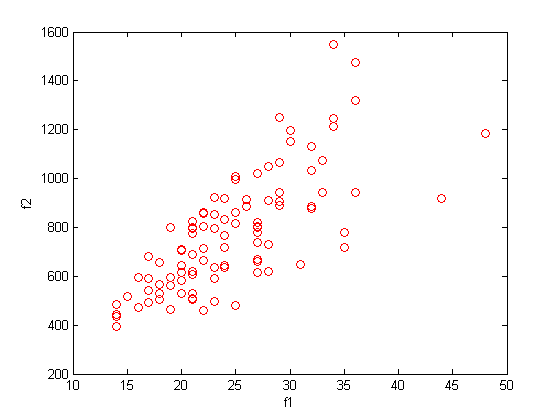
\includegraphics[width=8cm]{img/result-sp.png}
		\caption{Resultado da execução da soma ponderada com $\alpha = 0.1$.}
		\label{fig:result-sp}
	\end{figure}


\subsubsection{Otimização multiobjetivo - $\epsilon$-restrito}
Assim como nos algoritmos anteriores, o algoritmo implementado, utilizando a técnica do \emph{$\epsilon$-restrito}, para obter a solução do problema, precisa do parâmetro $\alpha$ do decaimento de temperatura. A partir das execuções dos algoritmos anteriores e de testes feitos durante a implementação, concluiu-se que o melhor valor seria $\alpha = 0.1$

Utilizando esse valor de $\alpha$, o script \texttt{epsilonRestrito.m} foi executado e o resultado pode ser visto a seguir.

\begin{figure}[h]
	\centering
	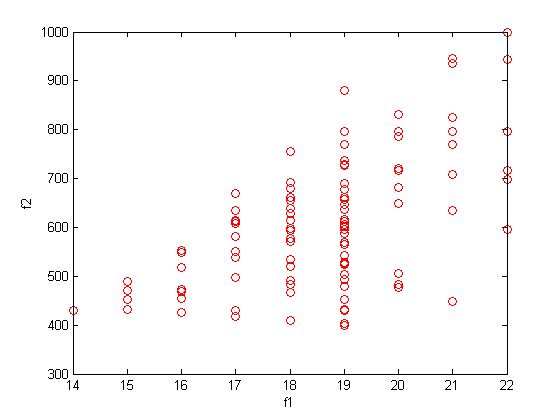
\includegraphics[width=7cm]{img/result-e.png}
	\caption{Soluções pareto-ótimas obtidas através do $\epsilon$-restrito}
	\label{fig:result-e}
\end{figure}
\newpage
A partir do gráfico da figura \ref{fig:result-e} é possível verificar que a maior parte das 100 soluções se concentrou em torno dos valores 18 e 19 para $f_1$ (tempo total de entrega) e 500 para $f_2$ (soma ponderada dos atrasos e adiantamentos). Esse resultado pode ser explicado pelo fato de terem sido utilizados valores de $\epsilon$ aleatórios, com distribuição normal, o que faz com que as soluções fiquem concentradas no centro da região das soluções pareto-ótimas. Ainda sim, foi obtida uma solução com valor 14 para $f_1$ e em torno de 400 para $f_2$, o que pode ser considerado um bom resultado.	

\subsubsection{Programação de Compromisso}

O teste do algoritmo da programação de compromisso é muito similar aos das implementações de problemas multiobjetivo anteriores. Também foi utilizado o parâmetro $\alpha = 0.1$ e o resultado pode ser visto a seguir.

\begin{figure}[h]
	\centering
	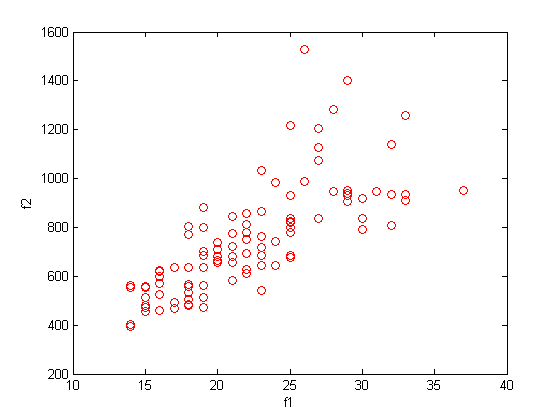
\includegraphics[width=7cm]{img/result-pc.png}
	\caption{Soluções obtidas através da programação de compromisso}
	\label{fig:result-pc}
\end{figure}

A partir da figura \ref{fig:result-pc} é possível visualizar que as soluções ficaram mais concentradas próximas dos valores 14 para $f_1$ e 400 para $f_2$. Isso de deve ao fato de esses serem parâmetros definidos como aceitáveis para as funções objetivo. É possível concluir então que o resultado está dentro do esperado.

\section{Conclusão}
Os métodos de otimização desenvolvidos neste trabalho foram sobretudo baseados no Simulated Annealing, que é um método de otimização não exato, contudo de fácil implementação e de desempenho satisfatório. É notável no decorrer do presente relatório que existem variações nas soluções encontradas. O Simulated Annealing é um ótimo método de estimação
de bons ótimos locais, no entanto ele não garante o ótimo global. Levando tudo isto em consideração, conclui-se que os resultados obtidos foram satisfatórios, considerando-se o desempenho e a qualidade das soluções encontradas.

\begin{thebibliography}{1}

\bibitem{notas de aula}
Notas de aula do professor Lucas Batista da disciplina \emph{ELE088 Teoria da Decisão}. 2017.

\bibitem{livro}
ARENALES, Marcos et al. Pesquisa operacional: para cursos de engenharia. Rio de Janeiro: Elsevier, 2007

\end{thebibliography}


% that's all folks
\end{document}


